%! Author = joels
%! Date = 24/12/2020

\section{Heap Memory Management}
% You can safely use heap allocation
% You can write leak free recursive data structures
% You can explain the difference between the two main smart pointers found in the STL
Don't do it yourselfe: Always rely on library classes for managing it (if possible).

\subsection{When is Heap Memory used}
\begin{itemize}
    \item Stack memory is scarce
    \item Might be needed for creating object structures
    \item Polymorphic factory functions to class hierarchies
\end{itemize}

\subsection{Heap Memory Legacy}
\textcolor{red}{Don't do that.} C++ allows allocating objects on the heap directly.\\
If done manually, you are responsible for deallocation and risk undefined behaviour:
\begin{itemize}
    \item Memory leaks
    \item Dangling pointers
    \item Double deletes
\end{itemize}

No garbage collection happens, it is your responsibility.

\begin{lstlisting}[style=frame, style= linenumbers, language=C]
// Don't use new / delete
auto ptr = new int{};
std::cout << *ptr << '\n';
delete ptr;
\end{lstlisting}

\subsection{Modern Heap Memory Management}
With the following smart pointers you don't have to call \textit{delete ptr;} yourself.\\
\textbf{Still:} Prefer storing a value locally as value-type variable
\subsubsection{std::unique\_ptr\textless T\textgreater}
\begin{itemize}
    \item Used for unshared heap memory
    \item For local stuff that must be on the heap (rare)
    \item Can be returned from a factory function
    \item Only a single owner exists
    \item Not best for class hierarchies (use \textit{std::shared\_ptr})
    \item Can not be copied
\end{itemize}
\vspace{1em}
Use-Cases:
\begin{itemize}
    \item As member variable
    \begin{itemize}
        \item To keep a polymorphic reference instantiated by the class or passed in as \textit{std::unique\_ptr} and transferring ownership
    \end{itemize}
    \item As local variable
    \begin{itemize}
        \item To implement RAII (Resource Acquisition Is Initialization)
        \item Can provide custom deleter function as second template argument
    \end{itemize}
    \item \textit{std::unique\_ptr\textless T\textgreater const p\{new\{\}\}}
    \begin{itemize}
        \item Cannot transfer ownership
        \item Cannot leak
    \end{itemize}
\end{itemize}
\begin{lstlisting}[style=frame, style= linenumbers, language=C]
// Factory
std::unique_ptr<X> factory(int i) {
    return std::make_unique<X>(i);
}
\end{lstlisting}

\pagebreak

\subsubsection{std::shared\_ptr\textless T\textgreater}
\begin{itemize}
    \item Works more like Java's references
    \item It can be copied and passed around
    \item The last one ceasing to exist deletes the object
    \item \textit{std::make\_shared\textless T\textgreater} allows T's public constructor's parameter to be used
\end{itemize}

\vspace{1em}

Use-Cases:
\begin{itemize}
    \item If you need heap-allocated objects, because you create your own object networks
    \item To support run-time polymorphic container contents or class members that can not be passed as reference
    \item Factory functions returning \textit{std::shared\_ptr} for heap allocated objects
    \item First check if alternatives are available
    \begin{itemize}
        \item (const) references as parameter types or class members
        \item Plain member objects or containers with plain class instances
    \end{itemize}
\end{itemize}

\begin{lstlisting}[style=frame, style= linenumbers, language=C]
struct A { /* constructor of A */ }
// Factory
auto createA() {
    return std::make_shared<A>(5, "hi", 'a');
}
int main() {
    auto anA = createA();
    auto sameA = anA; // second pointer to same obj
    A copyA{*sameA}; // copy ctr
    auto another = std::make_shared<A>(copyA); // copy ctr on heap
}
\end{lstlisting}

\subsubsection{Problem: Cyclic shared-Pointer Structures}
Usually, the last shared-Pointer handle destroyed will delete the allocated object.\\
Cyclic shared-Pointer structures keep themselfe alive, if they have circular dependencies to each other. Even if initial shared-Pointer handles are destroyed.
$\rightarrow$ \textit{std::weak\_ptr} breaks such cycles

\subsubsection{std::weak\_ptr \textless T\textgreater}
\begin{itemize}
    \item The \textit{shared\_ptr} cycles need to be broken
    \item \textit{weak\_ptr} does not allow direct access to the object
    \item A \textit{weak\_ptr} does not know weather the pointee is still alive
    \item \item with \textit{lock()} a \textit{shared\_ptr} to the object can be acquired if alive
\end{itemize}
\begin{center}
    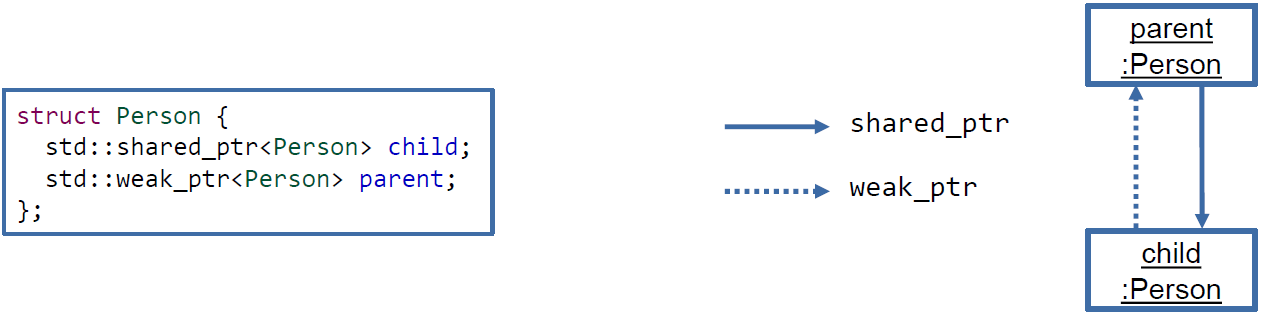
\includegraphics[width=0.6\linewidth]{weak_ptr.png}
\end{center}






























